\documentclass{article}
\usepackage{hw_style}
\usepackage{enumerate}
\usepackage{graphicx}
\usepackage{verbatim}

% Homework Specific Information
\newcommand{\hmwkTitle}{Homework \#1}
\newcommand{\hmwkDueDate}{Friday Sept. 30th}
\newcommand{\hmwkAuthorName}{Kurt Rudolph}%Name:
\newcommand{\hmwkNetID}{rudolph9}%your netid
\newcommand{\hmwkNotes}{}%I worked with...

\newcommand{\hmwkSubTitle}{}
\newcommand{\hmwkClass}{CS 412}
\newcommand{\hmwkClassTime}{Wed, Fri 3:30PM - 4:45PM}
\newcommand{\hmwkClassInstructor}{Jiawei Han}

\begin{document}
\begin{spacing}{1.1}
\maketitle
%=============================Problemi=========================%
\newpage
\begin{homeworkProblem}
	As a highly application-driven discipline, data mining has been widely applied in many areas. We brie�y presented two highly successful and popular application examples of data mining: business intelligence and Web search engines, in our textbooks. Do you think that data mining can also be applied to the following areas? If yes, please provide a brief yet concrete example, if not, please briefly state your reasons.
	
	\begin{enumerate}[(1)]
		\item Software Engineering
			\begin{homeworkSection}{Solution}
				Software Engineering often requires months and even years of development time to develop a single application.  Generally the projects involve a multitude of individuals and identifying where a the time of the development teams is being spent is an important when estimating completion dates and tracking completion of the various components.  Data mining can be applied to the discipline of software engineering by tracking development trends.  A real world example of this is the Atlassian Packages (Confluence being the wiki package currently utilized by the CS department here at UIUC).  
			\end{homeworkSection}
		\item Transportation
			\begin{homeworkSection}{Solution}
				The area of transportation can apply data mining to information collected on the various vehicles they use to provide service.  Trends can be identified to busses being late or early, the times of the day in which a train arrives late.  The information could be used to counteract the problems and provide better service to patrons.  
			\end{homeworkSection}
		\item Sociology
			\begin{homeworkSection}{Solution}
				Data mining may be applied to the area of sociology by identifying how persons interact with on another.  A good example is Facebook, what people like, who people are friends with, when people post, etc. are all tracked.  Methods of data mining can be applied to all information collected and identify various tends in human behavior.  
			\end{homeworkSection}
	\end{enumerate}
\end{homeworkProblem}
%=============================Problem2==========================%	
\begin{homeworkProblem}
	Suppose a student collected the price and weight of 20 products in a shop with the following result\\
	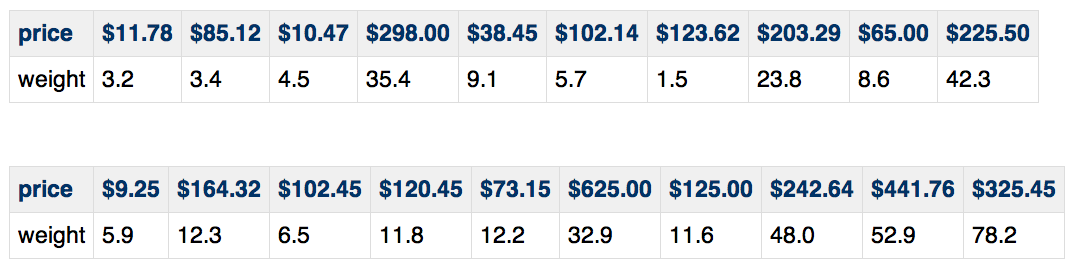
\includegraphics[width=\linewidth]{prob2.png}
	\begin{enumerate}[(1)]
		\item Calculate the mean, Q1, median, Q3, and standard deviation of price and weight
			\begin{homeworkSection}{Solution}
		
			\end{homeworkSection}
		\item Draw the boxplots for price and weight
			\begin{homeworkSection}{Solution}
		
			\end{homeworkSection}
		\item Draw scatter plot and Q-Q plot based on these two variables
			\begin{homeworkSection}{Solution}
		
			\end{homeworkSection}
		\item Normalize the two variables based on the min-max normalization $(min = 1, max = 10)$
			\begin{homeworkSection}{Solution}
		
			\end{homeworkSection}
		\item Normalize the two variables based on the z-score normalization
			\begin{homeworkSection}{Solution}
		
			\end{homeworkSection}
		\item Calculate the Pearson correlation coefficient. Are these two variables positively or negatively correlated?
			\begin{homeworkSection}{Solution}
		
			\end{homeworkSection}
		\item Take the price of the above 20 products, partition them into four bins by each of the following methods
			\begin{itemize}
				\item equal-width partitioning
				\item equal-depth (equal-frequency) partitioning
			\end{itemize}
				\begin{homeworkSection}{Solution}
		
				\end{homeworkSection}
	\end{enumerate}
\end{homeworkProblem}
%=============================Problemi==========================%	
\begin{homeworkProblem}
	Design a data warehouse for a university's gradebook data to analyze the class performances.  Suppose the data warehouse consisting of the following dimensions: department, semester, course, student, instructor, and gradebook; and a set of measures you would like to define.
	\begin{enumerate}[(a)]
		\item Draw a star-schema, based on your consideration of power and convenience of analysis of the warehouse
			\begin{homeworkSection}{Solution}
		
			\end{homeworkSection}
		\item Suppose we want to present the standard-deviation of final scores by course and year, and freely drilling up and down in multidimensional space, describe how this measure can be computed efficiently
			\begin{homeworkSection}{Solution}
		
			\end{homeworkSection}
		\item Is top 10\% in a class a holistic or algebraic measure?  Discuss how to develop an efficient (maybe approximate) methods to compute a query like: find those Engineering students whose final score is within top 10\% in class in at least 80\% of the CS courses that he or she has taken? 
			\begin{homeworkSection}{Solution}
		
			\end{homeworkSection}
		\item Is it a good idea to merge this data warehouse and the current university's gradebook database system together into one big data management/analysis system? Why?
			\begin{homeworkSection}{Solution}
		
			\end{homeworkSection}
	\end{enumerate}
\end{homeworkProblem}
%=============================Problemi==========================%	
\begin{homeworkProblem}
	A location-based social networking website which provides check-in services hires you to help them build a data warehouse. 

	Users of this service can "check-in" at venues using mobile device applications by running the applications and selecting from a list of venues that the application locates nearby. Also, users can "add" each other as "friends". The website also has sufficient information about venues, including address, GPS location, and category of the venue (e.g., a Japanese restaurant), and users tend to provide their personal information to the website when they register.
	\begin{enumerate}[(a)]
		\item Design a data warehouse that may facilitate effective on-line analytical processing for this website (provide both schema and measures, also explain why).
			\begin{homeworkSection}{Solution}
		
			\end{homeworkSection}
		\item Check-in data collected from the website and mobile applications are noisy. Besides network and device errors, are there any other reasons which might cause noises in this data set? For the reason you come up with, discuss a method that can clean-up check-in data effectively in the data warehouse.
			\begin{homeworkSection}{Solution}
		
			\end{homeworkSection}
		\item One may like to performance on-line analytical processing to the checks-in data at different venues by month, by cities and by categories (Italian or Japanese, etc.). How can this be done efficiently in the data warehouse?
			\begin{homeworkSection}{Solution}
		
			\end{homeworkSection}
		\item Hackers create fake profiles on this website. They are using bots to manipulate fake profiles, generate fake check-in data and try to add everyone as their friends (yes this is a common problem for many social network websites, and no, I am not telling you how to write bots). Although bots are trying to mimic real users, they still behave differently, e.g., they check-in at random places (Chicago this minute, Las Vegas next minute), they check-in way too often than real users, and their social network structures are usually very large but also very sparse (your friends on facebook tend to form communities but bots don't do that). Discuss possible solutions on how to identify fake profiles (bots) in your data warehouse.
			\begin{homeworkSection}{Solution}
		
			\end{homeworkSection}
	\end{enumerate}
\end{homeworkProblem}
	
\end{spacing}
\end{document}

\begin{comment}%==========================================================
%=============================Problemi==========================%	
\begin{homeworkProblem}
	
	\begin{homeworkSection}{Solution}
		
	\end{homeworkSection}
\end{homeworkProblem}
%=============================Problemi==========================%	
\begin{homeworkProblem}
	
	\begin{enumerate}[(a)]
		\item 
			\begin{homeworkSection}{Solution}
		
			\end{homeworkSection}
	\end{enumerate}
\end{homeworkProblem}
%=============================Problemi==========================%	
\begin{homeworkProblem}
	{\bf }	
	\begin{homeworkSection}{Solution}
		
	\end{homeworkSection}
\end{homeworkProblem}
%=============================Problemi==========================%	
\newpage
\begin{homeworkProblem}
	{\bf  }	
	\begin{enumerate}[(a)]
		\item 
			\begin{homeworkSection}{Solution}
		
			\end{homeworkSection}
	\end{enumerate}
\end{homeworkProblem}
%=============================Problemi=========================%
\newpage
\begin{homeworkProblem}
	
	\begin{homeworkSection}{Solution}
		
	\end{homeworkSection}
\end{homeworkProblem}

\end{comment}%=========================================================
















